\documentclass[10pt,a4paper,twoside,twocolumn]{revtex4-1}
\usepackage{fontspec}
\defaultfontfeatures{Mapping=tex-text}
\usepackage{xunicode}
\usepackage{xltxtra}
%\setmainfont{???}
\usepackage{amsmath}
\usepackage{amsfonts}
\usepackage{amssymb}
\usepackage{float}
\usepackage{subcaption}
\begin{document}
\title{Review of the benchmarks}
\maketitle
\section{Benchmark 1:}
We consider the $1D$ model on a PBC lattice of $L$ sites described by the Hamiltonian
\begin{equation}
H=\sum_{i=1}^L \left[ \sigma^{x}_{i} \sigma^{x}_{i+1} + \sigma^{y}_{i} \sigma^{y}_{i+1} + \sigma^{z}_{i} \sigma^{z}_{i+1}\right], 
\end{equation}
where $\{\sigma^{x}_i,\sigma^{y}_i,\sigma^{z}_i\}^{L}_{i=1}$ are the $\{x,y,z\}$ Pauli matrices on the site $i$, and where because of PBC $\sigma^{a}_{L} \sigma^{a}_{L+1} = \sigma^{a}_{L}\sigma^{a}_{1}$.\\
\subsection{Notation for the datasets and choice of monomials} 
The data of Jie are computed for different choices of the set of monomials, the notation is as follows ($a,b,c,e=x,y,z$):
\begin{table}[H]
\label{tab:notation-B1}
\begin{tabular}{ |l|l| }
\hline
\textbf{notation} & \textbf{monomials}\\
\hline
\textbf{d=$2$} & $1$, $\sigma^{a}_i$, $\sigma^{a}_i\sigma^{b}_{i+1}$\\
\hline
\textbf{d=$3$} & $1$, $\sigma^{a}_i$, $\sigma^{a}_i \sigma^{b}_{i+1}$, $\sigma^{a}_i \sigma^{b}_{i+1} \sigma^{c}_{i+2}$ \\
\hline
\textbf{d=$3$ extra} & $1$, $\sigma^{a}_i$, $\sigma^{a}_i \sigma^{b}_{i+1}$, $\sigma^{a}_i \sigma^{b}_{i+1} \sigma^{c}_{i+2}$, $\sigma^{a}_i \sigma^{b}_{i+2}$ \\
\hline
\textbf{d=$4$} & $1$, $\sigma^{a}_i$, $\sigma^{a}_i \sigma^{b}_{i+1}$, $\sigma^{a}_i \sigma^{b}_{i+1} \sigma^{c}_{i+2}$, $\sigma^{a}_i \sigma^{b}_{i+1} \sigma^{c}_{i+2} \sigma^{e}_{i+3}$\\
\hline
 \textbf{d=$4$ extra} & $1$, $\sigma^{a}_i$, $\sigma^{a}_i \sigma^{b}_{i+1}$, $\sigma^{a}_i \sigma^{b}_{i+1} \sigma^{c}_{i+2}$, $\sigma^{a}_i \sigma^{b}_{i+1} \sigma^{c}_{i+2} \sigma^{e}_{i+3}$, \\
 &  $\sigma^{a}_i \sigma^{b}_{i+2}$, $\sigma^{a}_i \sigma^{b}_{i+3}$, $\sigma^{a}_i \sigma^{b}_{i+1} \sigma^{c}_{i+3}$, $\sigma^{a}_i \sigma^{b}_{i+2} \sigma^{c}_{i+3}$\\
\hline
\end{tabular}
\end{table}
The parameter $d$ specify the degree of the monomials considered, the term \textit{"extra"} specify the inclusion of the lower degree monomials with operators at $d-1$ maximum distance.\\
Further studies has been done for different choices of the monomials, for example in subsection \ref{par:parameter-r} we study the dependence of the our approximations from the addition of monomials of degree $2$ of operators at distance $\leq r$, where $r$ was the parameter we were varying, i.e. the addition of the mononomials $\sigma^{a}_{i}\sigma^{b}_{i+k}$ with $1<k\leq r$. We obtained an imporovement of the lower bound of the GS energy (as expected from the theory), but no apparent correlations between the value of $r$ and the quality of the approximation of other quantities as the correlators.
 

\subsection{GS Energy}

The gound state energy lower bounds computed with $d>2$ are closer to the exact value with respect to the ones obtained with similar method in \cite{baumgratz2012} (they differ from us in the fact that they mapped the spin system to fermions, while we work directly with spins) and with respect to the ones computed with variational methods \cite{haim2020}.

\begin{figure}[H]
  \centerline{
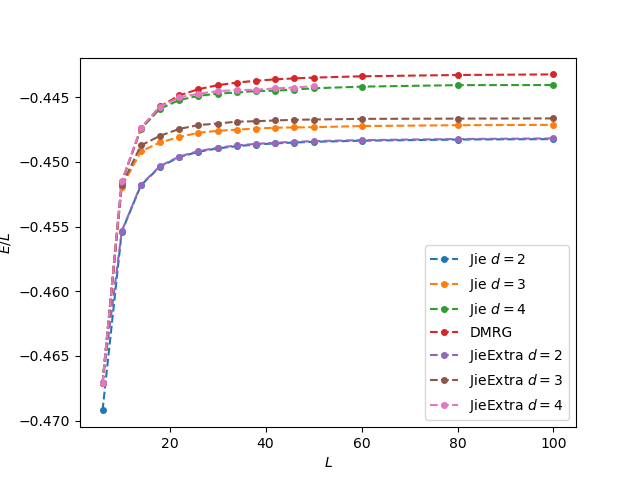
\includegraphics[width=1.\linewidth]{Figures/B1/Energies-d4-Extra.png}}
  \captionof{figure}{Values of the lower bound on the energy computed with the SDP methods compared with the (approximately exact) DMRG value. We notice that the lower bound improves as we increase the value of the $d$ parameter, while it is less sensitive to the inclusion of the "extra" monomials.}
  \label{Fig:GSE-B1}
\end{figure}

\textbf{Energies $\rightarrow$ Good!}

\subsection{Correlations}

\begin{figure}[H]
  \centerline{
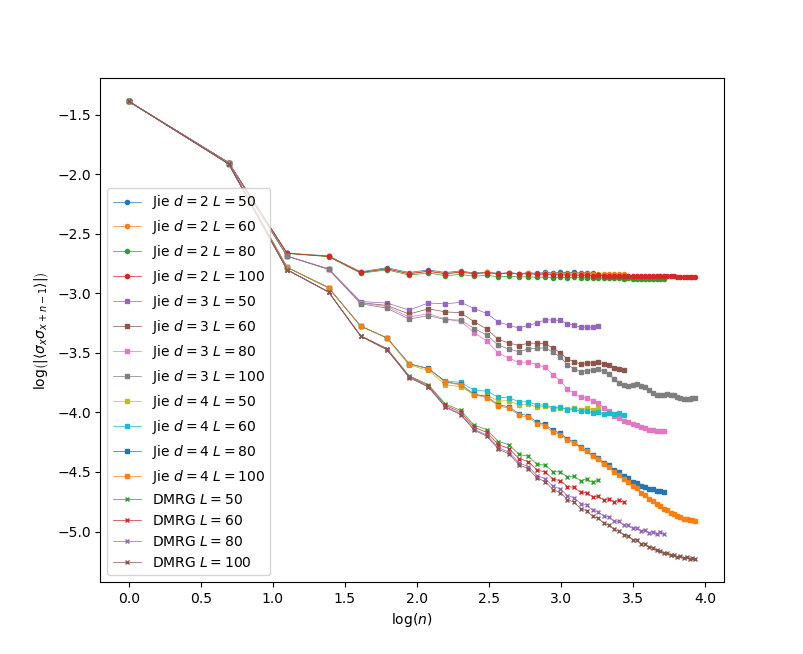
\includegraphics[width=1.\linewidth]{Figures/B1/Correlations_log-log-d4.png}}
  \captionof{figure}{Log-Log plot for the decay of correlations for different dimensions $L$ and different parameters for the SDP. From the DMRG calculations we expect the correlations to decay as a power law.}
  \label{Fig:Power-Law-Correlations-B1}
\end{figure}
In figure \ref{Fig:Power-Law-Correlations-B1} we plot the decays of correlations in log-log scale for different dimensions $L$ and different parameters of the SDP. From the DMRG calculations we expect the correlations to decay as a power law. We see that the SDP with $d=2$ is not able to capture the qualitative behaviour of the decay of the correlations saturating to a plateau. For bigger values of $d$ the SDP start capturing the right qualitative behaviour, getting better as $d$ increase and as $L$ increase.

\begin{figure}[H]
  \centerline{
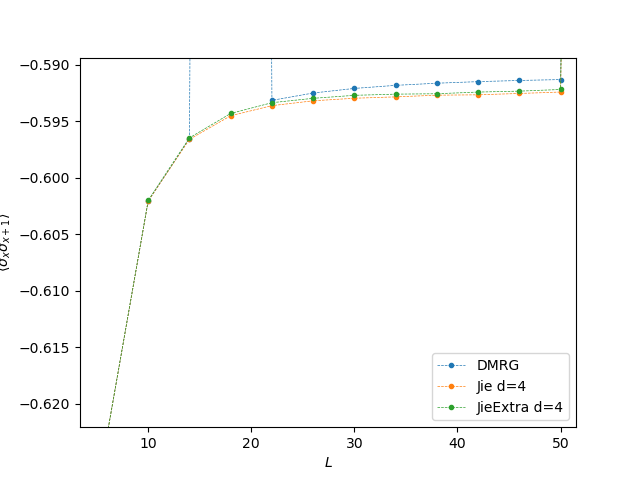
\includegraphics[width=1.\linewidth]{Figures/B1/_Baumgratz_FIG._2_right_below-d4-Extra.png}}
  \captionof{figure}{First nearest neighbour correlator as a function of system size $L$. The SDP calculations appear to lower bound the value of the first nearest neighbour correlator. }
  \label{Fig:Power-Law-Correlations-bottom-B1}
\end{figure}
\begin{figure}[H]
  \centerline{
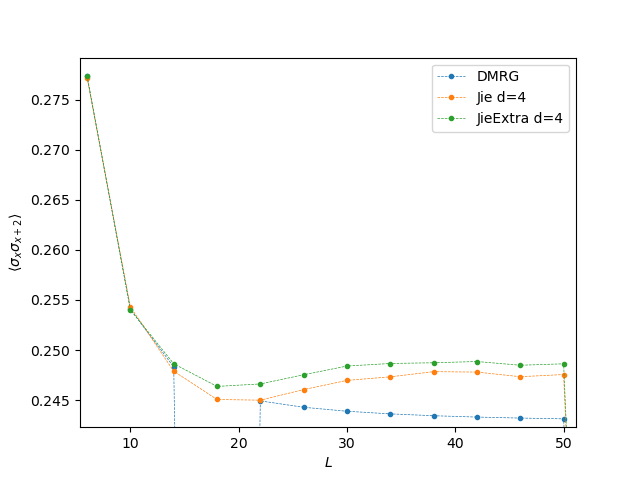
\includegraphics[width=1.\linewidth]{Figures/B1/_Baumgratz_FIG._2_right_up-d4-Extra.png}}
  \captionof{figure}{Second nearest neighbour correlator as a function of system size $L$. The SDP calculations appear to upper bound the value of the second nearest neighbour correlator.}
  \label{Fig:Power-Law-Correlations-top-B1}
\end{figure}

In figures \ref{Fig:Power-Law-Correlations-bottom-B1} and \ref{Fig:Power-Law-Correlations-top-B1} we plot the first and second nearest neighbours as a function of the system size $L$. It is possible to make a direct comparison with the right panel of FIG. 2. in \cite{baumgratz2012}  where the same quantities are plotted. We see that with our method we obtain far better results in estimatiting the first nearest neighbour correlators (\ref{Fig:Power-Law-Correlations-bottom-B1}) both for small systems (where our lower bound is almost tight w.r.t. the exact results) and for larger systems (where our method seems to saturate to a fixed distance from the exact value). 
In the case of the second nearest neighbour correlators (\ref{Fig:Power-Law-Correlations-top-B1}) our method returns qualitatively different results from the one of Baumgratz and Plenio. In fact, while for small systems the computed value are almost exact, for larger $L$, the behaviour of $\langle \sigma_x \sigma_{x+2} \rangle$ with $L$ changes and the predicted values seems to not converge to the exact one, making a impossible to use the method for a scaling dimension analysis. Comparing the numerical values, though, our method seems to be as good as the one we are comparing it to (please note the different scale on the vertical axis).
It is interesting to note that the lower bound both for first and second nearest neighbour improves increasing the value of $d$.

\textbf{Correlations $\rightarrow$ Good!}

\subsection{Structure factor}


\begin{figure}[H]
  \centerline{
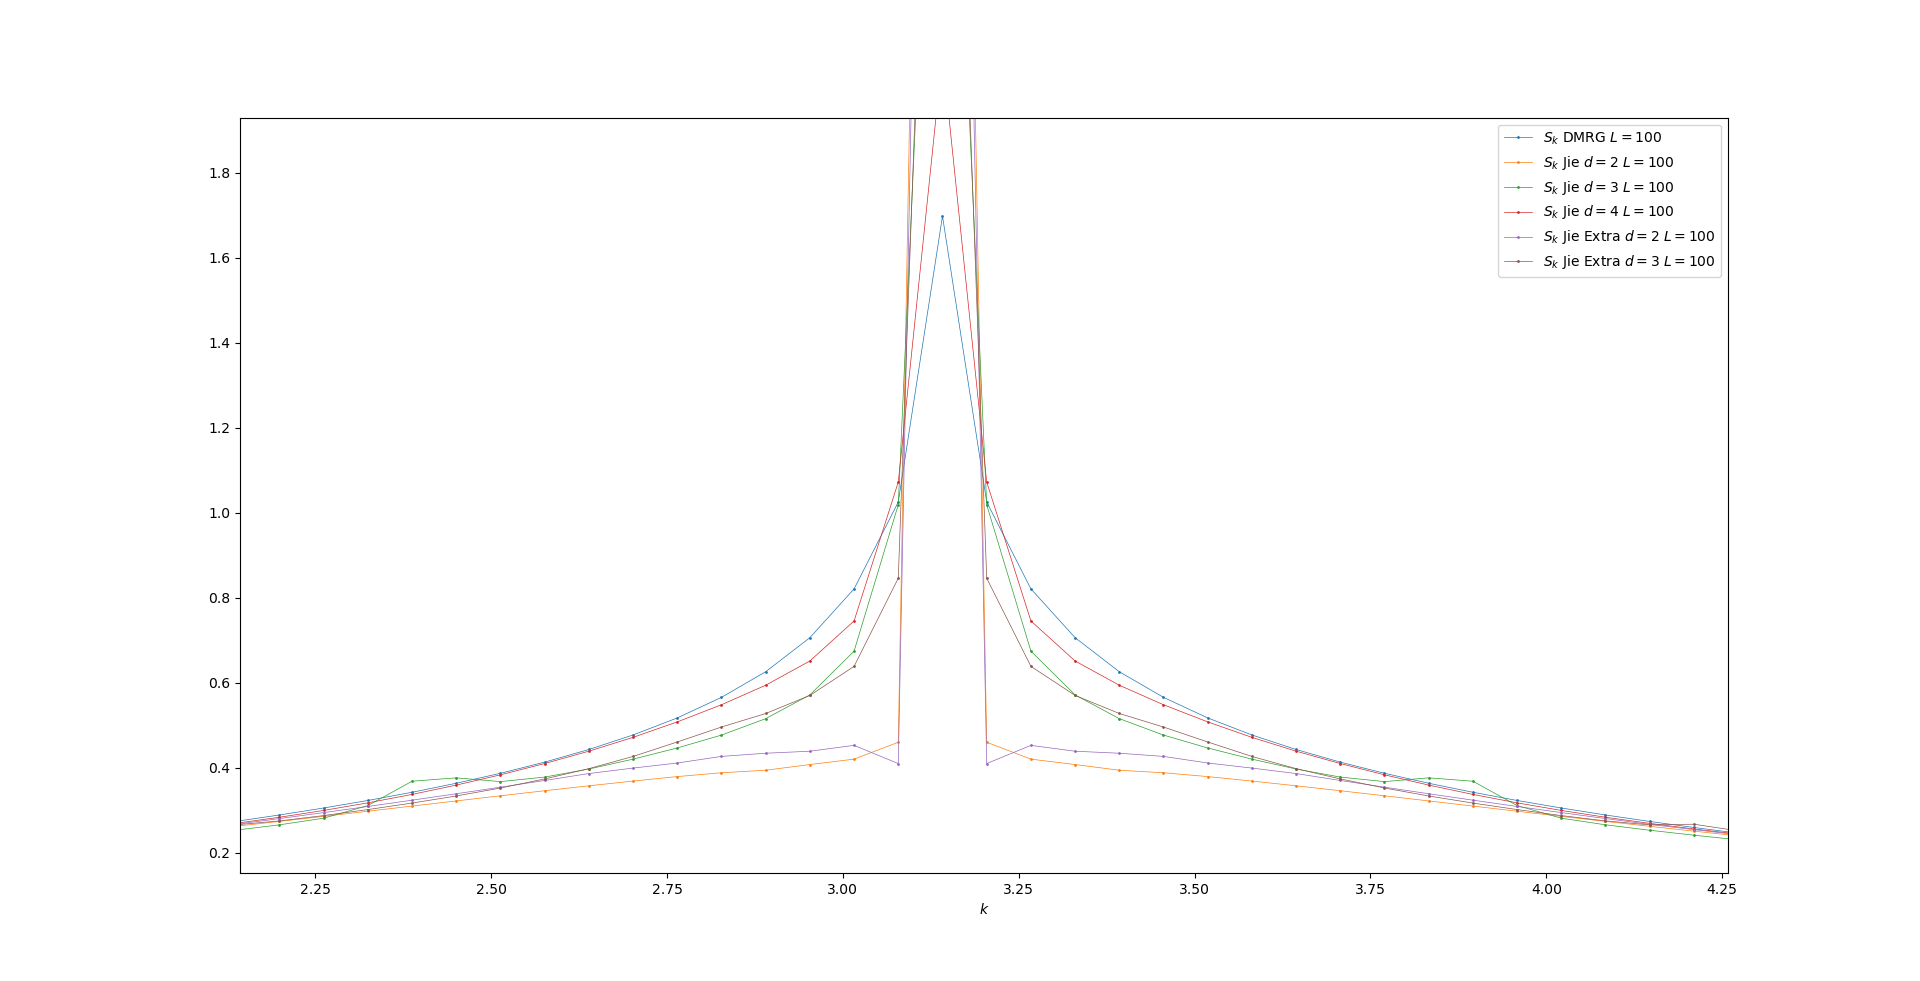
\includegraphics[width=1.\linewidth]{Figures/B1/Struncture_factor-zoom.png}}
  \captionof{figure}{Structure factor for system size $L=100$.}
  \label{Fig:Structure-factor-total-B1}
\end{figure}
\begin{figure}[H]
  \centerline{
\includegraphics[width=1.\linewidth]{Figures/B1/Size_scaling_at_π_-_log-log_scale.png}}
  \captionof{figure}{Value of the structure factor at $\pi$ vs the size of the system in log-log scale. }
  \label{Fig:Structure-factor-pi-B1}
\end{figure}
\begin{figure}[H]
  \centerline{
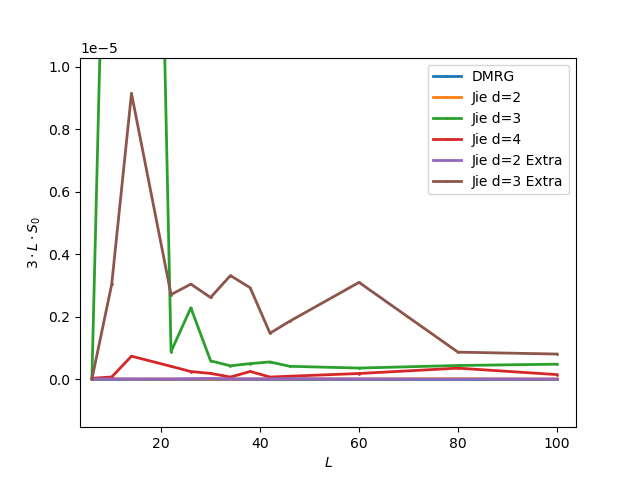
\includegraphics[width=1.\linewidth]{Figures/B1/Size_scaling_at_0.png}}
  \captionof{figure}{Value of the structure factor at $0$ vs the size of the system. Note the scale on the vertical axis.}
  \label{Fig:Structure-factor-0-B1}
\end{figure}

In figures \ref{Fig:Structure-factor-total-B1}, \ref{Fig:Structure-factor-pi-B1}, \ref{Fig:Structure-factor-0-B1} we study the approximated values of the structure factor  $S_k$ computed from the SDP data with the (exact) one computed with DMRG method.\\
The values of the structure factor are really sensitive to the long distance correlations. \\
From the theory we expect for $S_{k=\pi}$ to behave as a power low with respect to the size of the system $L$ for which is computed, while we expecte $S_{k=0}$ to be proportional to the expectation value of the square of the total spin, that in our case is $0$, so we expect it to be close to $0$. \\
From figure \ref{Fig:Structure-factor-pi-B1} we notice that even for $d=4$ the structure factor does not clearly scale as a power law with the system size as hoped, while for smaller values of $d$ it is clear that the SDP approximation is not constrained enough to reproduce the expected qualitative behaviour of $S_{k=\pi}$.
Surprisingly, we see that, in the case of $S_{k=0}$ the SDP approximation is able to reproduce the expected behaviour for all values of $d$. This implies that that the global information about the rotational symmetry has been implicitly encoded in the SDP formulation without the necessity of explicitly imposing the global constraint.

\textbf{Structure factor $\rightarrow$ partially good.}

\subsection{Inclusion of longer distance monomials} 
\label{par:parameter-r}
For the SDP approximation we use the set of monomials specified in table \ref{tab:notation-B1}. Here each set of monomials was specified just by the parameter $d$, the maximum degree of the  monomial considered. The maximum distance $r$ between the support of each operator in the monomials was dependent on $d$. Here we study what happens if we relax this constraint and let $r$ vary independently. In particular we study how the approximations with $d=4$ vary with addition of the mononomials $\sigma^{a}_{i}\sigma^{b}_{i+k}$ with $1<k\leq r$ to the set of monomials $d=4$. 
\begin{figure}[H]
  \centerline{
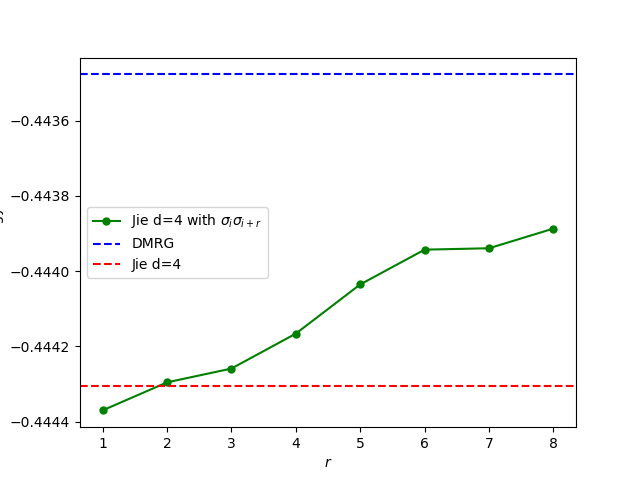
\includegraphics[width=1.\linewidth]{Figures/B1/L=50,_r_parameter.png}}
  \captionof{figure}{Ground state energy computed for a system of size $L$ for different values of $r$.}
  \label{Fig:GSE-r-B1}
\end{figure}
In figure \ref{Fig:GSE-r-B1} we see that increasing $r$ improves the lower bound on the ground state energy (as expected). Similarly the approximated value of the first nerest neighbour correlator improves with $r$ (see figure \ref{Fig:NN-corr-r-B1}), while the quality of the approximation of the second nerest neighbour correlator seems to not be correlated with $r$ (see figure \ref{Fig:NextNN-corr-r-B1}).
\begin{figure}[H]
  \centerline{
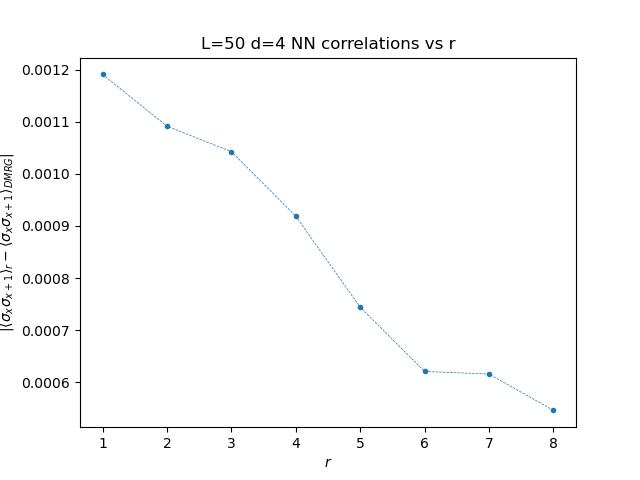
\includegraphics[width=1.\linewidth]{Figures/B1/NN_correlations_L=50.png}}
  \captionof{figure}{Difference between first nearest neighbour correlator computed with DMRG and computed with SDP for $d=4$ and varying parameter $r$. The SDP values improves with growing $r$.}
  \label{Fig:NN-corr-r-B1}
\end{figure}

\begin{figure}[H]
  \centerline{
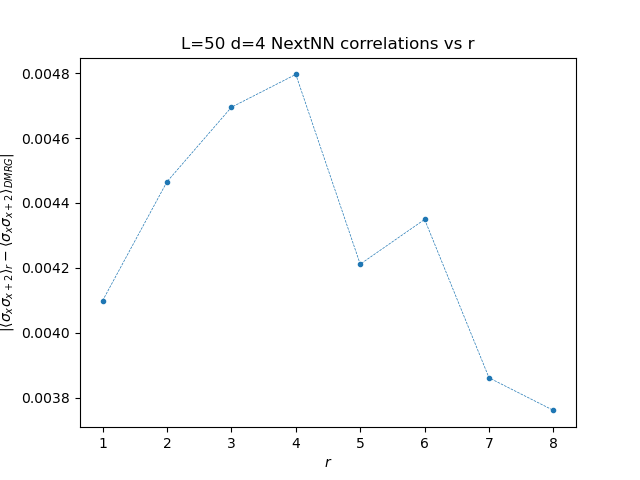
\includegraphics[width=1.\linewidth]{Figures/B1/NextNN_correlations_L=50.png}}
  \captionof{figure}{Difference between second nearest neighbour correlator computed with DMRG and computed with SDP for $d=4$ and varying parameter $r$. There seems to not be any correlation between the quality of the approximation and $r$.}
    \label{Fig:NextNN-corr-r-B1}
  \end{figure}
  \textbf{Longer distance monomials $\rightarrow$} unfortunately, including longer distance monomials seems to not be directly correlated to the improvements of the approximations of (not obvious) quantities.
  
  
\subsection{Physicality of the reduced density matrices}
 From the value of the correlators in the moment matrix we can recover the full reduced density matrices $\rho_A$ of all the systems up to dimension $|A|=2*d$, where $d$ is the parameter of the SDP approximation.
 Having the reduced density matrices allows us to verify if the moment matrix describes physical marginals. A moment matrix with physical $k$-body marginals, lower bounds the GS energy by a value lower bounded by the $k$-body marginals Anderson bound. That is, it would be a sure improvement of the $k$-bopdy marginals Anderson bound.\\
 The correlation matrices for $d=4$ have physical $2$-body marginals, but the $4$-body marginals are already not-physical. This is a good news. We can adopt and hybrid Anderson-SDP strategy and impose the positivity of the $4$-body marginals (and even for the $k$-body marginals, with $k>4$) in the SDP and expect for an improvement of the bound.
 
The constraint corresponding to the $k$-body physicality is
\begin{equation}
\frac{1}{2^k} \left( 1 + \sum_{\vec{x}} \langle \sigma^{x_1}_{1}\sigma^{x_2}_{2}\dots \rangle \sigma^{x_1}_{1}\sigma^{x_2}_{2}\dots \right) \geq 0 ,
\end{equation}
a positive constraint linear in the moments,  where $\vec{x}$ are all the $k$ elements vectors, where each element $x_i \in \{0,1,2,3\}$ and $\sigma^{0}_{i}=\mathbb{I}_{i},$ $\sigma^{1}_{i}=\sigma^{x}_{i},$ $\sigma^{2}_{i}=\sigma^{y}_{i},$ $\sigma^{3}_{i}=\sigma^{z}_{i},$.

Note that we are not limited by the size of the moments in the NPA part. If the moments in the moment matrix are not enough to reconstruct the previous m-particle matrix, we introduce new variables and demand positivity of the resulting operator (still linear in the unknowns)

 
 \textbf{Phisicality $\rightarrow$} there is room for an hybrid Anderson-SDP approach. 
 
 
 
 \section{Benchmark 2:}
We consider the $J_1$-$J_2$ Heisenberg model on a $1D$ lattice with PBC
\begin{align}
 H  = & \sum_{i=1}^L \big[ J_1 \left( \sigma_i^x \sigma_{i+1}^x+\sigma_i^y \sigma_{i+1}^y+\sigma_i^z \sigma_{i+1}^z \right)+\\
& + J_2 \left( \sigma_i^x \sigma_{i+2}^x+\sigma_i^y \sigma_{i+2}^y+\sigma_i^z \sigma_{i+2}^z \right)  \big],
 \end{align}
 with $J_1=1$, and $J_2>0$. The choice of $J_2=0$ is the model of benchmark-$1$.
 For $J2/J1 = 0.5$ the hamiltonian has two GS namely the states in which neighboring pairs of spins form singlet configurations \cite{majumdar1969,white1996}.
 We compare the SDP results with the one computed from DMRG calculation. We consider the DMRG calculations exact.
We consider systems of linear dimensions $L=10,20,30,40$. The SDP calculations are able to give results for larger systems (i.e. we have some data for $L=50,100$), but DMRG calculations were stuck in some local minima making us unable to easily access larger systems.


\subsection{Notation for the datasets and choice of monomials}
The data of Jie are computed for different choices of the set of monomials, the notation is as follows ($a,b,c,e=x,y,z$):
\begin{table}[H]
\label{tab:notation-B1}
\begin{tabular}{ |l|l| }
\hline
\textbf{notation} & \textbf{monomials}\\
\hline
\textbf{d=$2$} & $1$, $\sigma^{a}_i$, $\sigma^{a}_i\sigma^{b}_{i+1}$, $\sigma^{a}_i\sigma^{b}_{i+2}$\\
\hline
\textbf{d=$2$ extra} & $1$, $\sigma^{a}_i$, $\sigma^{a}_i\sigma^{b}_{i+1}$, $\sigma^{a}_i\sigma^{b}_{i+2}$, $\sigma^{a}_i\sigma^{b}_{i+3}$\\
\hline
\textbf{d=$3$} & $1$, $\sigma^{a}_i$, $\sigma^{a}_i \sigma^{b}_{i+1}$, $\sigma^{a}_i\sigma^{b}_{i+2}$, $\sigma^{a}_i \sigma^{b}_{i+1} \sigma^{c}_{i+2}$ \\
\hline
\textbf{d=$3$ extra} & $1$, $\sigma^{a}_i$, $\sigma^{a}_i \sigma^{b}_{i+1}$, $\sigma^{a}_i\sigma^{b}_{i+2}$, $\sigma^{a}_i \sigma^{b}_{i+1} \sigma^{c}_{i+2}$, $\sigma^{a}_i\sigma^{b}_{i+3}$ \\
\hline
\textbf{d=$4$} & $1$, $\sigma^{a}_i$, $\sigma^{a}_i \sigma^{b}_{i+1}$, $\sigma^{a}_i\sigma^{b}_{i+2}$, $\sigma^{a}_i \sigma^{b}_{i+1} \sigma^{c}_{i+2}$, $\sigma^{a}_i \sigma^{b}_{i+1} \sigma^{c}_{i+2} \sigma^{e}_{i+3}$\\
\hline
 \textbf{d=$4$ extra} & $1$, $\sigma^{a}_i$, $\sigma^{a}_i \sigma^{b}_{i+1}$, $\sigma^{a}_i\sigma^{b}_{i+2}$, $\sigma^{a}_i \sigma^{b}_{i+1} \sigma^{c}_{i+2}$, $\sigma^{a}_i \sigma^{b}_{i+1} \sigma^{c}_{i+2} \sigma^{e}_{i+3}$, \\
 &  $\sigma^{a}_i \sigma^{b}_{i+3}$, $\sigma^{a}_i \sigma^{b}_{i+1} \sigma^{c}_{i+3}$, $\sigma^{a}_i \sigma^{b}_{i+2} \sigma^{c}_{i+3}$\\
\hline
\end{tabular}
\end{table}

The difference w.r.t. table \ref{tab:notation-B1} is that, to be consistent with always including all the monomials present in the Hamiltonian, here we always include $\sigma^{a}_i\sigma^{b}_{i+2}$ for all values of $d$ and we include $\sigma^{a}_i\sigma^{b}_{i+3}$ as extra term.

 
\subsection{GS Energy} 
The quality of the lower bound on the GS energy seems to not improve with the size of the system, but improves significantly including the extra terms.
\begin{figure}[H]
  \centerline{
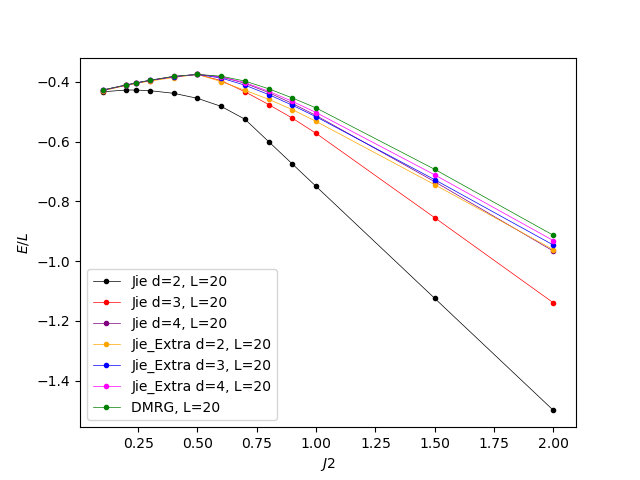
\includegraphics[width=1.\linewidth]{Figures/B2/Energies_L=20.png}}
  \captionof{figure}{Ground state energies computed for a system of size $L=20$ with SDP method and DMRG as a function of the Hamiltonian's parameter $J_2$. SDP results are labelled using the notation of table \ref{tab:notation-B1}.}
  \label{Fig:GSE-L20-B2}
\end{figure}
\begin{figure}[H]
  \centerline{
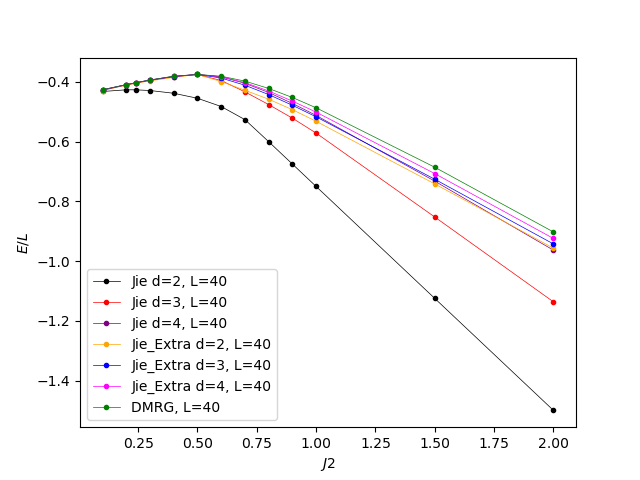
\includegraphics[width=1.\linewidth]{Figures/B2/Energies_L=40.png}}
  \captionof{figure}{Ground state energies computed for a system of size $L=40$ with SDP method and DMRG as a function of the Hamiltonian's parameter $J_2$. SDP results are labelled using the notation of table \ref{tab:notation-B1}.}
  \label{Fig:GSE-L40-B2}
\end{figure}
\begin{figure}[H]
  \centerline{
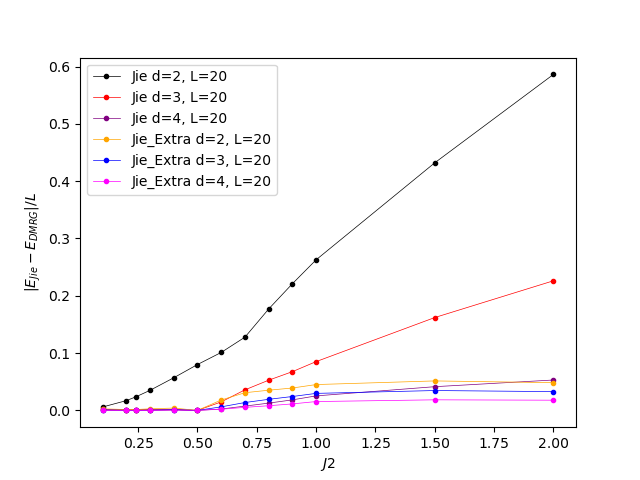
\includegraphics[width=1.\linewidth]{Figures/B2/Energy_differences_L=20.png}}
  \captionof{figure}{Difference between the GS energy computed with SDP method and DMRG as a function of the Hamiltonian's parameter $J_2$ for the system of dimension $L=20$. }
  \label{Fig:Delta-GSE-L20-B2}
\end{figure}
\begin{figure}[H]
  \centerline{
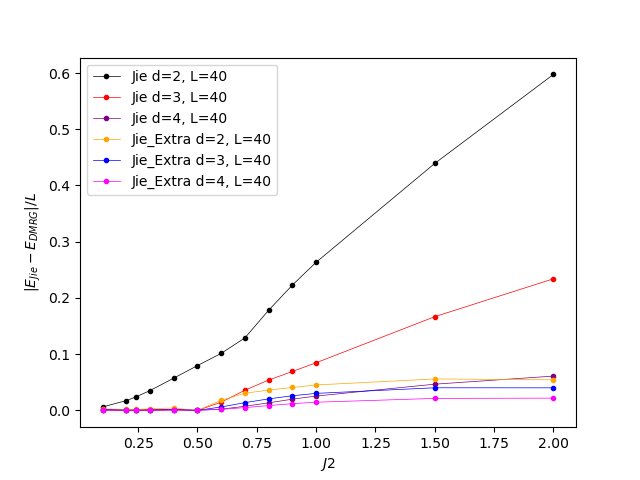
\includegraphics[width=1.\linewidth]{Figures/B2/Energy_differences_L=40.png}}
  \captionof{figure}{Difference between the GS energy computed with SDP method and DMRG as a function of the Hamiltonian's parameter $J_2$ for the system of dimension $L=40$. }
  \label{Fig:Delta-GSE-L40-B2}
\end{figure}


\subsection{Structure factor}
From the theory we know that for the structure factor there should be a peak at $k=\pi$, which for $J_2>0.5$ is moving towards $k=\frac{\pi}{2}$ for $J_2 = \infty $ \cite{chitra1995}.
This behaviour is evident in figure \ref{Fig:Structure-factor-DMRG-B2} where we plot the structure factor $S_{k}$ as a function of $k$ for a system of size $L=40$ for different values of the Hamiltonian's parameter $J_2$ from the DMRG data. \\
The same behaviour is reproduced also by the SDP data (see figure \ref{Fig:Structure-factor-SDP-B2}). \\

Comparing the two figures we can see how the SDP method is not able to capture the special structure of the GS at $J_2=\dfrac{1}{2}$. The structure factor computed from the DMRG data with $J_2=\dfrac{1}{2}$ is constant for every value of $k$,  a sign that the correlations in the ground states are peacked (indeed we know that at $J_2=\dfrac{1}{2}$ the GS is a product state of singlets). The structure factor computed from the SDP data does not encode this information, indeed looking at the values of the correlators, the SDP methods returns long distance correlations.

\begin{figure}[H]
  \centerline{
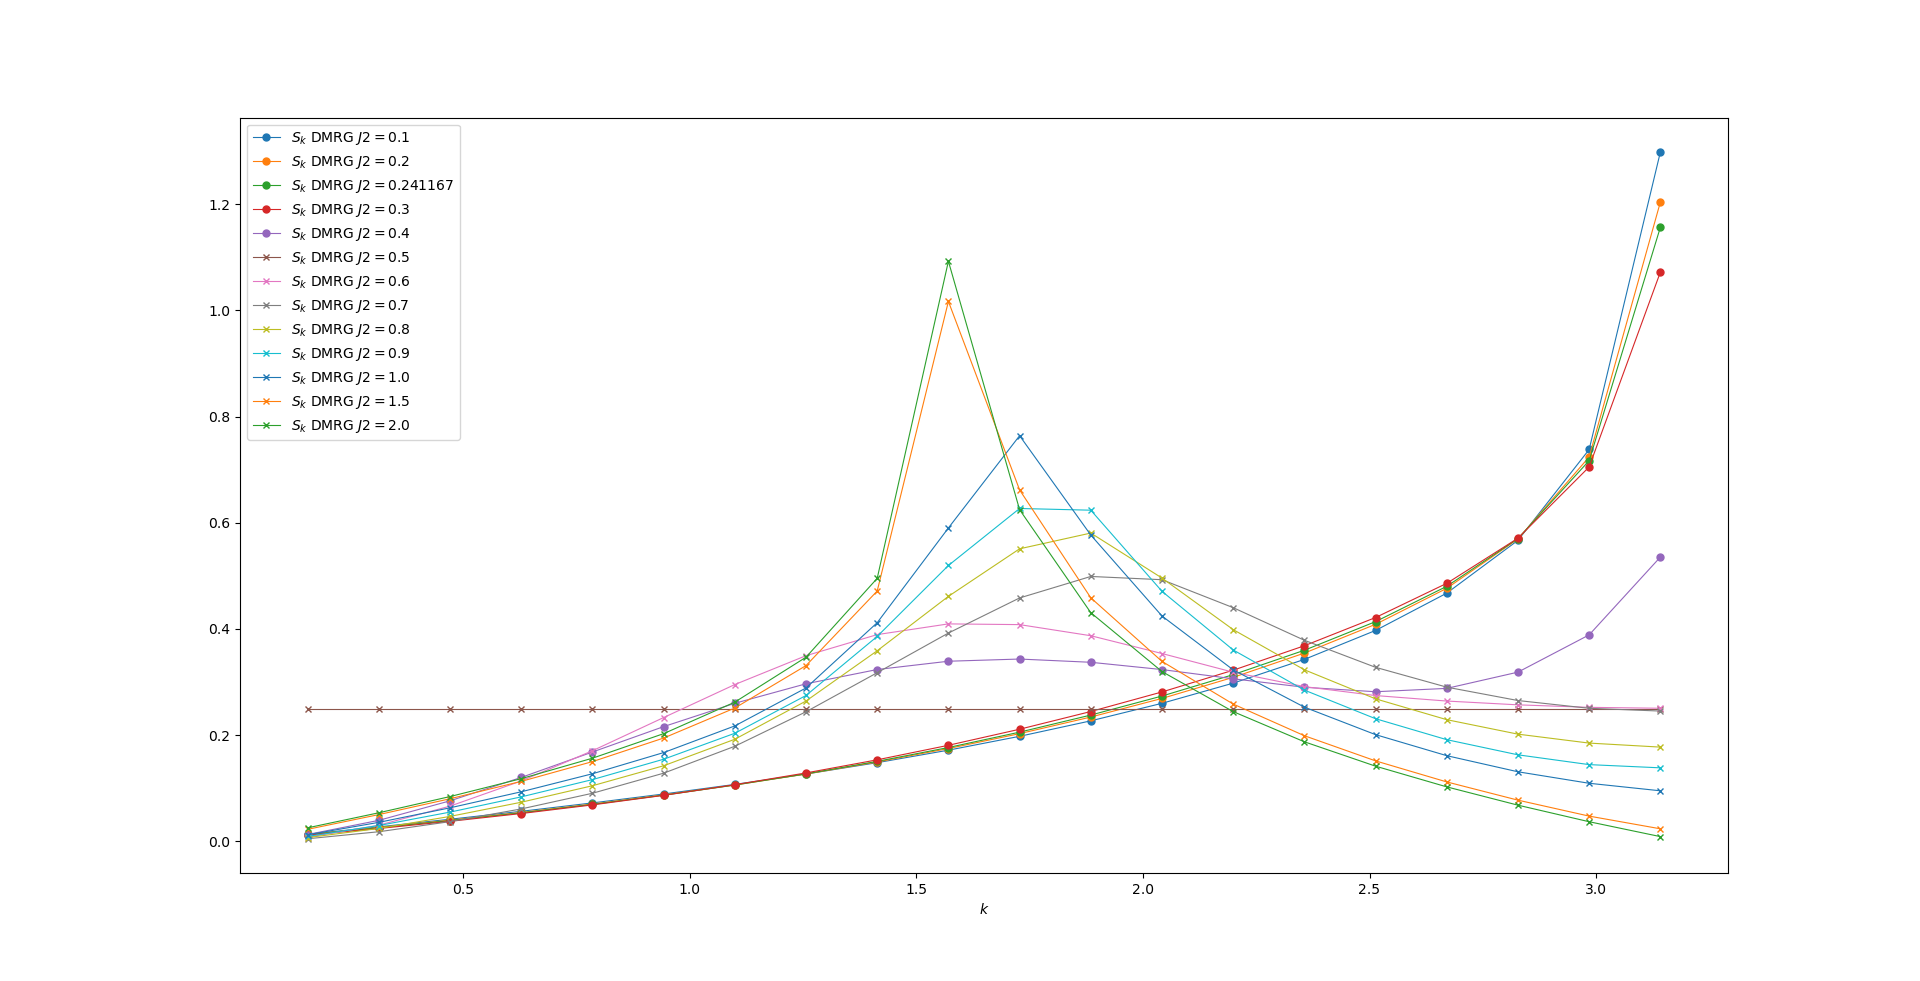
\includegraphics[width=1.\linewidth]{Figures/B2/Struncture_factor_DMRG.png}}
  \captionof{figure}{Structure factor $S_{k}$ as a function of $k$ for a system of size $L=40$ computed for different values of the Hamiltonian's parameter $J_2$ from the DMRG data. }
  \label{Fig:Structure-factor-DMRG-B2}
\end{figure}
\begin{figure}[H]
  \centerline{
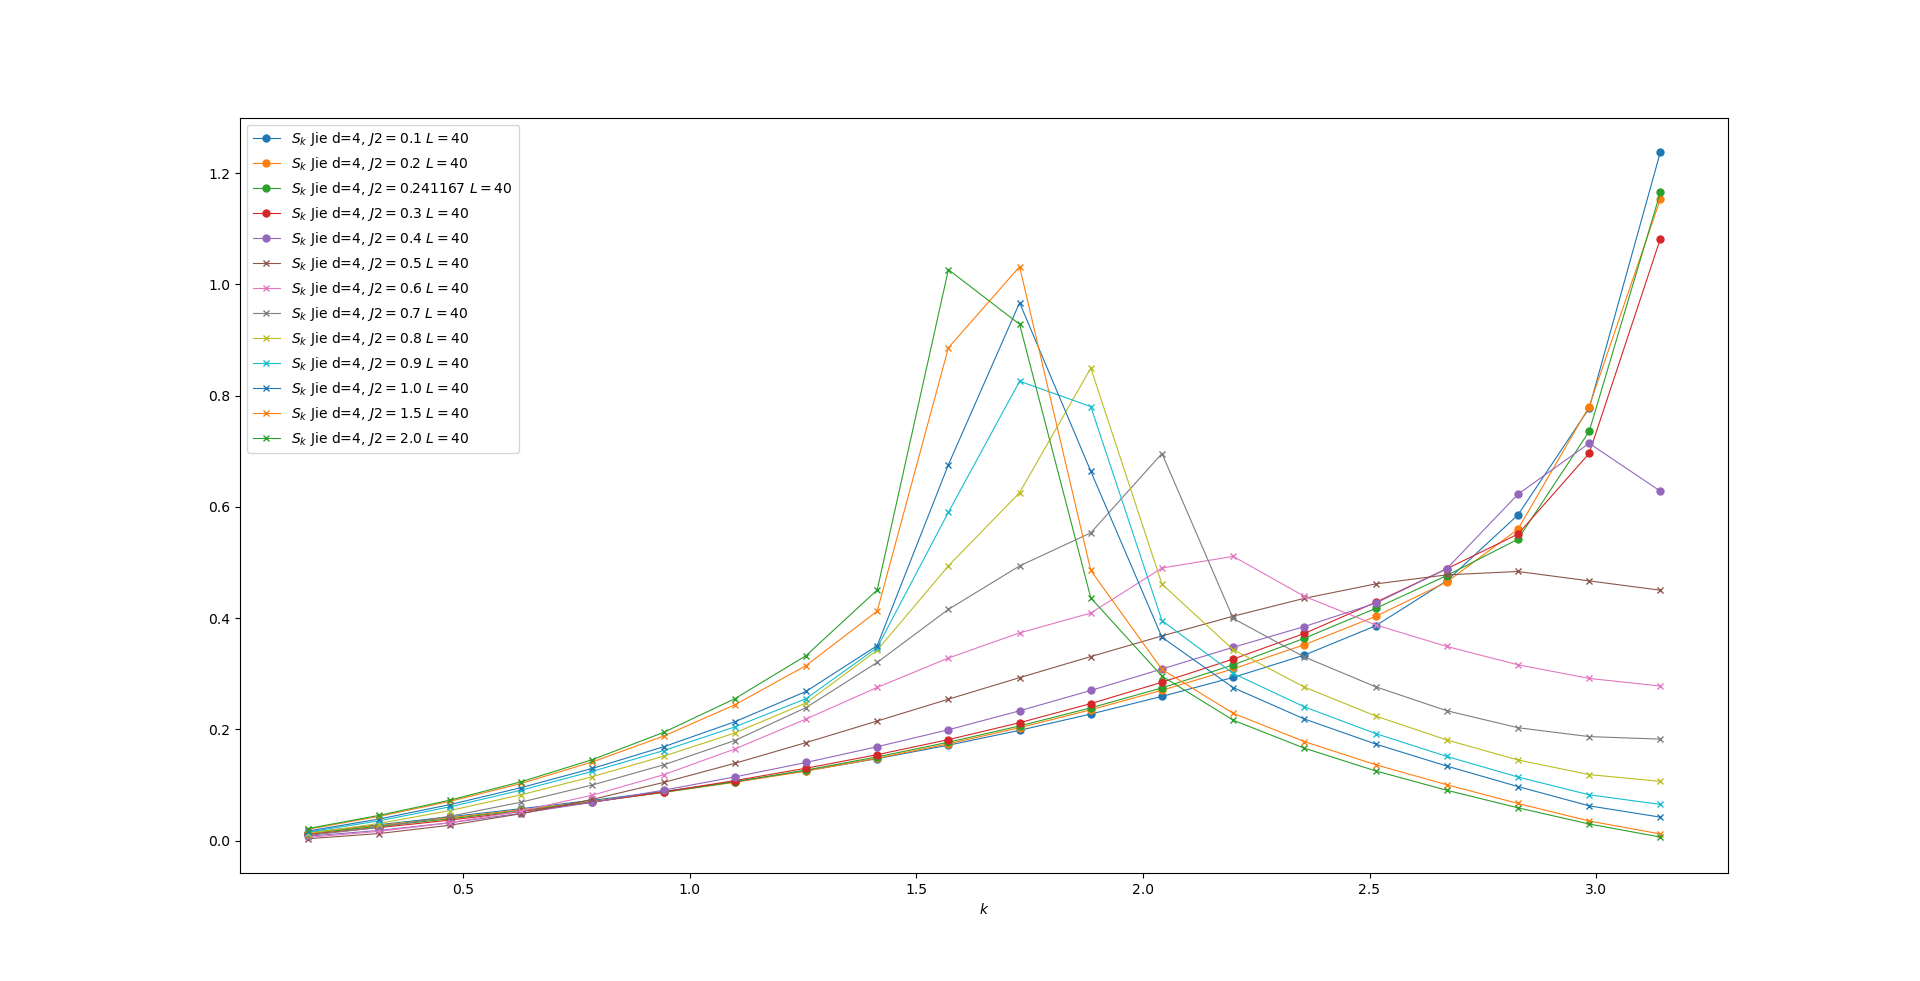
\includegraphics[width=1.\linewidth]{Figures/B2/Struncture_factor_Jie.png}}
  \captionof{figure}{Structure factor $S_{k}$ as a function of $k$ for a system of size $L=40$ computed for different values of the Hamiltonian's parameter $J_2$ from the SDP data with $d=4$.}
  \label{Fig:Structure-factor-SDP-B2}
\end{figure} 

\textbf{Structure factor $\rightarrow$ partially good.}


\bibliography{GSESDP.bib}
\bibliographystyle{ieeetr}

\end{document}
